\documentclass[border=3pt,tikz]{standalone}
\usepackage[utf8]{vietnam}
\usetikzlibrary{calc,angles,intersections,shapes.geometric,arrows,decorations.markings,arrows.meta,patterns.meta,patterns}
\usepackage{tikz-3dplot,pgfplots}
\pgfplotsset{compat=1.15}
\usepgfplotslibrary{polar}
\usepackage{amsmath}
\begin{document}
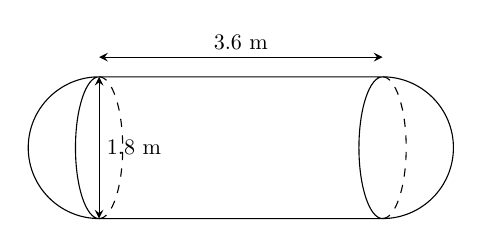
\begin{tikzpicture}[declare function={r=.9;}]% đặt các tham số bán kính
	\draw[dashed]
	(0:0) arc (-90:90:r/3 and r)
	(0:4*r) arc (-90:90:r/3 and r);
	\draw
	(0:0) arc (270:90:r)arc (90:270:r/3 and r)--(0:4*r) arc (-90:90:r)arc (90:270:r/3 and r)
	(90:2*r)--+(0:4*r);
	\draw[stealth-stealth] (90:2*r +.25)--+(0:4*r) node[midway,above,scale=.8]{$3.6$ m};
	\draw[stealth-stealth] (0:0)--(90:2*r) node[midway,right,scale=.8]{$1.8$ m};
\end{tikzpicture}
\end{document}
